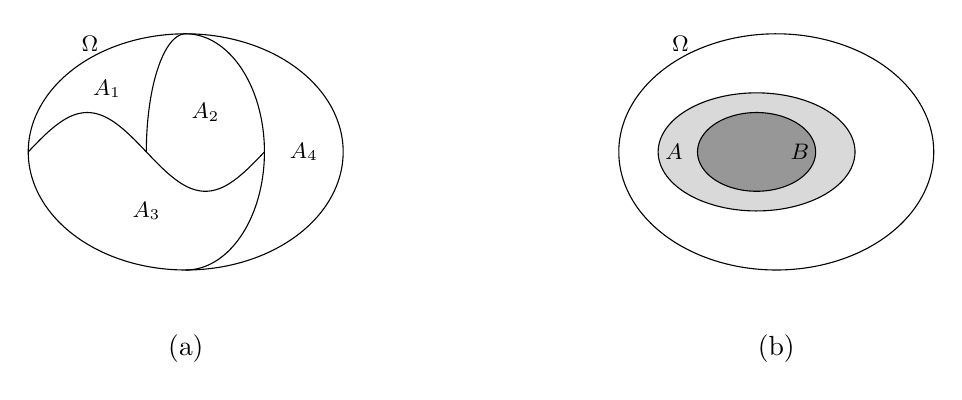
\begin{tikzpicture}%[scale=.9]
\shorthandoff{>}
%
% Particion
\begin{scope}
%
% Omega y A_i
\draw[domain=0:360,samples=200] plot ({2*cos(\x)+.5},{1.5*sin(\x)});
\draw[domain=-90:90,samples=200] plot ({cos(\x)+.5},{1.5*sin(\x)});
\draw[domain=90:180,samples=200] plot ({.5*cos(\x)+.5},{1.5*sin(\x)});
\draw[domain=0:3,samples=200] plot (\x-1.5,{.5*sin(120*\x)});
%
%
% Omega y A_i's
\draw(-.5,1.375) node[left,scale=.9]{\small $\Omega$};
\draw(-.5,.8) node[scale=.9]{\small $A_1$};
\draw(.75,.5) node[scale=.9]{\small $A_2$};
\draw(0,-.75) node[scale=.9]{\small $A_3$};
\draw(2,0) node[scale=.9]{\small $A_4$};
%
\draw (.5,-2.5) node{(a)};
\end{scope}
%
%
% Inclusion
\begin{scope}[xshift=7.5cm]
%
\fill[opacity=.15] plot[domain=0:360,samples=200] ({1.25*cos(\x)+.25},{.75*sin(\x)});
\fill[opacity=.3] plot[domain=0:360,samples=200] ({.75*cos(\x)+.25},{.5*sin(\x)});
%
% borders A, B y Omega
\draw[domain=0:360,samples=200] plot ({1.25*cos(\x)+.25},{.75*sin(\x)});
\draw[domain=0:360,samples=200] plot ({.75*cos(\x)+.25},{.5*sin(\x)});
\draw[domain=0:360,samples=200] plot ({2*cos(\x)+.5},{1.5*sin(\x)});
%
% A, B, Omega
\draw (-.8,0) node[scale=.9]{\small $A$};
\draw(.8,0) node[scale=.9]{\small $B$};
\draw(-.5,1.375) node[left,scale=.9]{\small $\Omega$};
%
\draw (.5,-2.5) node{(b)};
\end{scope}
%
\end{tikzpicture}